\documentclass[a4paper,12pt]{article}
\usepackage[utf8]{inputenc}
\usepackage[frenchb]{babel}
\usepackage{graphicx}
\usepackage[T1]{fontenc}
\usepackage{fancyhdr}
\usepackage{graphics}
\usepackage{verbatim}
\setcounter{page}{1}
\fancyhead[L]{\leftmark}
\fancyhead[R]{}

\fancyfoot[C]{}
\fancyfoot[R]{\thepage}



\begin{document}
\begin{titlepage}
		\newpage
		\thispagestyle{empty}
		\begin{center}
			
\includegraphics[scale=0.15]{images/logo_fac}	
		\end{center}
		\begin{center}
			\vspace{0.3cm}
			\large  
			\textbf{Mémoire de Master 2 MIAGE}\\
			\vspace{0.7cm} \large 
			\vskip 0.2in
		\end{center}
		\fbox{%
			\parbox{\textwidth}{%
				\begin{center}
					\begin{center}
						\large \textsc{\textbf{ Comment, à partir de la reconnaissance faciale et de la fouille de données, peut on identifier l’ensemble des sosies potentiels d’une personne ?  }}
					\end{center}
					
				\end{center}
			}%
		}
		\begin{center}
		    Application à l’univers du cosplay
		\end{center}
		
		\begin{flushleft}
			\begin{center}
			
					\textbf{Réalisé par} \\
					\hspace{0.1cm} VILLER Nathanaëlle \\
					\textbf{Tuteur}\\
				 \hspace{0.1cm} GUEHIS Sonia \\
			
			\end{center}
		\end{flushleft}
	
		\begin{center}
			\vspace{0.1cm} \textbf{Année scolaire 2017-2018}
		\end{center}
		
%\newpage
%\thispagestyle{empty}
%\section*{Remerciements}
 
\newpage
\tableofcontents
\thispagestyle{empty}
\end{titlepage}

\newpage
	\pagenumbering{arabic}
%\addcontentsline{toc}{section}{Introduction}
%\section*{Introduction}

%\textit{}
%\\ \\

%\newpage

\addcontentsline{toc}{section}{Glossaire}
\newpage
\section*{Glossaire}
\begin{description}
\item [Sosie :] Personne qui a une parfaite ressemblance avec une autre au point qu'on peut les confondre.
\item [Cosplay :] Le phénomène du cosplay a commencé dans les années 40 aux Etats Unis. Mais c'est lors des années 70 et 80 que le cosplay atteint son paroxysme grâce aux succès de Star Trek et Star Wars. Le Japon va ensuite adopter ce phénomène et lui donner le nom qu'il porte aujourd'hui : le cosplay (qui vient de la contraction de costume et playing). Le principe est simple : Il faut se déguiser en un personnage de fiction et incarner ce personnage. Le mouvement va s'intensifier au Japon et Tokyo deviendra le centre névralgique de ce phénomène. Il faudra attendre les années 90 pour que le cosplay arrive en Europe. La scène européenne se démarquera part sa volonté de respect du craft (fabrication manuel de son costume). Les conventions et concours vont se multiplier. Les cosplayers vont de plus en plus chercher de nouvelles techniques pour pouvoir ressembler le plus possible aux personnages qu'ils essaient d'incarner. Il y a 2 grandes catégories qui se démarquent. Ceux qui cosplay leurs personnages préférés sans se soucier de la morphologie et ceux qui essaie de trouver des personnages qui leur correspondent physiquement.
\item [Cosplayer :] n.m Peut s'écrire aussi cosplayeur, ou cosplayeuse pour les femmes. Il s'agit d'une personne pratiquant l'art du cosplay. 
\item [Cosplayer :] Verbe d'action signifiant l'art de pratiquer le cosplay. 

\end{description}

\addcontentsline{toc}{section}{Introduction}
\newpage
\section*{Introduction}
Quand on parle de sosie on pense généralement à la personne qui pourrait être notre jumeau. Mais si nous agrandissions le champ de recherche ? Au lieu de se limiter à des être humains réels nous pourrions chercher nos sosies dans le domaine du dessins animés, des peintures, des personnages de films, etc... 

Qu'existe-il actuellement pour permettre de trouver un sosie ? Comment fonctionne ces solutions ? Quels sont leurs limites ? 

Comment pourrions-nous agrandir ce champ de recherche et avoir des résultats plus fidèles ? Quels sont les contraintes ? 

Dans quel cadre cette solution pourrait-elle être utiliser et quand pense la population ? 
\\ \\
Ce mémoire à pour but de répondre à toutes ces interrogations.
\\ \\
En découle notre interrogation : comment, à partir de la reconnaissance faciale et de la fouille de données, peut on identifier l’ensemble des sosies potentiels d’une personne ?

\newpage
\section{Présentation de la problématique}
\subsection{Enquête}
La première étape de la recherche a été de mener une étude afin d'étudier la pertinence du sujet.
Cette dernière a permis d'avoir l'avis de 487 personnes sur le projet en question. L'étude a été réalisé via un google form et partagé sur Facebook et par mail. 
Voici quelques chiffres pour décrire les personnes ayant répondu à cette enquête : 
\begin{itemize}
    \item 79\% sont des femmes 
    \item 78\% ont entre 18 et 30 ans
    \item 13\% ont plus de 30 ans
    \item 75\% pratiquent le cosplay
    \item 37\% sont des artistes
    \item 21\% ne sont ni cosplayer ni artiste
\end{itemize}
Les chiffres utilisés dans ce mémoire, sauf précisions, proviennent donc de cette étude. 

\subsection{Vous avez dit sosies ?}
Lorsque nous parlons de sosie, la première image qui nous vient est une personne en tout point conforme à nos traits physiques avec qui nous pourrions échanger nos identités. Il existe de nombreuses oeuvres sur ce concept comme par exemple le "\textit{Le Prince et le Pauvre}", roman de Mark Twain publié en 1882 qui a eu plusieurs adaptation en film, où l'on voit un prince et un pauvre physiquement identique échanger de place. Ou bien "\textit{Deux pour le prix d'une}" roman de 1949 d'Erich Kästner qui a aussi connu des adaptations en films notamment par Disney. Le roman raconte une histoire entre 2 fillettes qui découvrent qu'en réalité elles sont soeurs jumelles et décident d'inverser leur place auprès de parents divorcés. Ou encore le drama coréen "\textit{Who Are You: School 2015}" sortie en 2015 qui raconte l'histoire de 2 soeurs, elles aussi jumelles, séparées à la naissance. Là aussi, une des soeurs va devoir usurper la place de l'autre afin de faire avancer l'intrigue. Ce genre d'histoire mêlant jumeaux et usurpation/échange d'identité est fréquente et le public en est friand. Nous voyons que ce phénomène n'est pas restreint ni à une époque ni à une culture. De plus, la recherche de sosies de personnalités connues est fréquente, exemple pour le tournage d'un film. 
\\ \\
Rechercher son sosie par curiosité, ou pour tout autre raison, même lorsque l'on n'a pas eu la chance de naître avec un jumeau est monnaie courante. Mais pourquoi se contenter de chercher uniquement parmi les être humains ? Et si un personnage fictif pouvait nous ressembler ? Si un personnage d'une série, d'un dessin, de jeux vidéo ou même une peinture pouvait nous ressembler ? Et si l'on pouvait analyser des photos pour récupérer tous les personnages fictifs nous ressemblant en prenant en compte le style graphique de chaque oeuvre ? Aimeriez-vous avoir accès facilement à une liste de personnages qui vous ressemble ? 82,83\% des personnes sondées disent que oui. 
\\ \\

\subsection{Cas d'application}
70,84\% des cosplayers font parfois attention à cosplayer un personnage qui a une morphologie proche de la leur. Et parmi eux, un peu moins de la moitié trouve cela important et y font attention. Bien que le cosplay soit un loisir où chacun doit se sentir libre d'incarner le héros de son choix, on voit qu'il y a une forte tendance chez les cosplayer à faire attention à la similitude entre eux et les personnages choisis. 
\\ \\
Bien qu'environ 83\% des cosplayers fonctionnent au "coup de coeur" et choisissent leur projet cosplay parmi les personnages qu'ils connaissent et leur plaisent. Ils sont tout autant à avoir répondu qu'ils seraient intéressés à accéder à une liste de personnages leur ressemblant. Ce projet n'est pas nécessaire à la pratique cosplay mais permettrait d'ouvrir de nouveaux champs d'étude, en effet la réalisation de cosplay ne se ferait plus que sur des personnages connus à l'avance. Mais au contraire serait un point d'accès pour découvrir un nouvel univers. Cela se ressant dans les commentaires renseignés lors de l'étude : avoir accès à une liste de personnage leur ressemblant permettrait de "favoriser le choix de costume par rapport à notre corps, pour les rendre plus approprié", mais encore que "c'est une bonne chose, cela peut permettre d'avoir plus de possibilité" ou alors peut être "très bien pour les gens ayant du mal à faire un choix ou n'ayant pas d'idée", ... Donc, proposer une liste de personnage ressemblant à la photographie d'une personne, serait une amélioration dans la communauté cosplay.  

\subsection{Problématique}
80,29\% des personnes ayant été sondés (donc pas uniquement les cosplayers) ont répondus être intéressées d'utiliser une application permettant de récupérer une liste de sosies, dans le cadre du cosplay mais aussi du déguisement. De plus, à peine 6,16\% trouvait l'idée mauvaise ou plutôt mauvaise. 

Pour le développement d'une telle application nous pourrions nous baser en premier lieu sur la reconnaissance faciale, puis agrandir le champ à la reconnaissance morphologique pour la comparaison d'image et ainsi repérer les sosies. 
Afin d'avoir un ensemble de données suffisant à une telle recherche, il serait intéressant d'ajouter des logiciels de type "crawler" afin d'obtenir l'ensemble du champ d'application du web pour l'étude. 

Le sujet mérite donc d'être approfondit. 

\textit{Comment, à partir de la reconnaissance faciale et de la fouille de données, peut-on identifier l'ensemble des sosies potentiels d'une personne ? }
\section{État de l'art}
Dans un premier temps, il convient d'étudier les solutions existantes pouvant en partie ou complètement à cette problématique. 
L'objectif est de trouver une solution permettant de renseigner en entrée une photographie/image et d'obtenir à partir de celle ci, une image/photographie similaire à celle ci. De plus, nous souhaitons pouvoir comparer la morphologie ainsi que des caractéristiques physiques tel que la couleur de peau, la couleur des yeux ou la couleur des cheveux. Et tout cela, en parcourant le plus grand nombre de résultat possible, issu directement de la toile. Et enfin, les images en retours ne doivent pas être uniquement des photographies de personnes réelles.

\subsection{Solutions existantes et limites}
\subsubsection{Moteurs de recherches par mots clefs}
Les moteurs de recherchent par mots clefs ne sont pas pertinents dans le cadre de notre recherche, ces derniers ne permettent pas d'avoir un retour suffisamment précis et clair et sont déjà très étudiés et répandu. 
\subsubsection{Les moteurs de recherches d'images inversées}
Les moteurs de recherches d'images inversées permettent de mettre en entrée une image et en sortie de lister tous les sites utilisant cette image. Cela ne correspond pas à ce que nous cherchons. Mais l'algorithme utilisé pour parcourir le web à la recherche de tous les sites utilisant une image peut être intéressant. 
\subsubsection{Recherche par couleur}
Des sites proposent de mettre en entrée des couleurs et en sorties de lister des images possédant les couleurs en question. En fonction des sites les images peuvent posséder d'autre couleurs ou n'ont que celles sélectionnées, comme par exemple sur le site labs.tineye.com/multicolr. Cela ne correspond pas non plus à notre recherche. 
\subsubsection{Google Image}
Google est connu pour permettre la recherche par mot clef. Mais il permet aussi de mettre en entrée une image pour trouver les images similaires. Faisons l'expérience avec 2 images très différentes. La première provient d'une recherche par mots clefs sur Google Image (Figure 1) et la seconde est une photographie de moi dont je suis l'auteur (Figure 2). 
    \begin{figure}[!h]
    \centering
        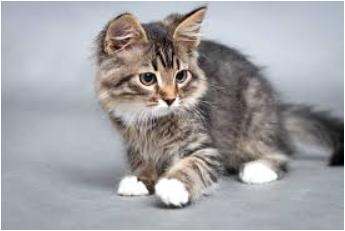
\includegraphics[scale=0.7]{images/telechargement.PNG}
        \caption{Chat de Google Images}
        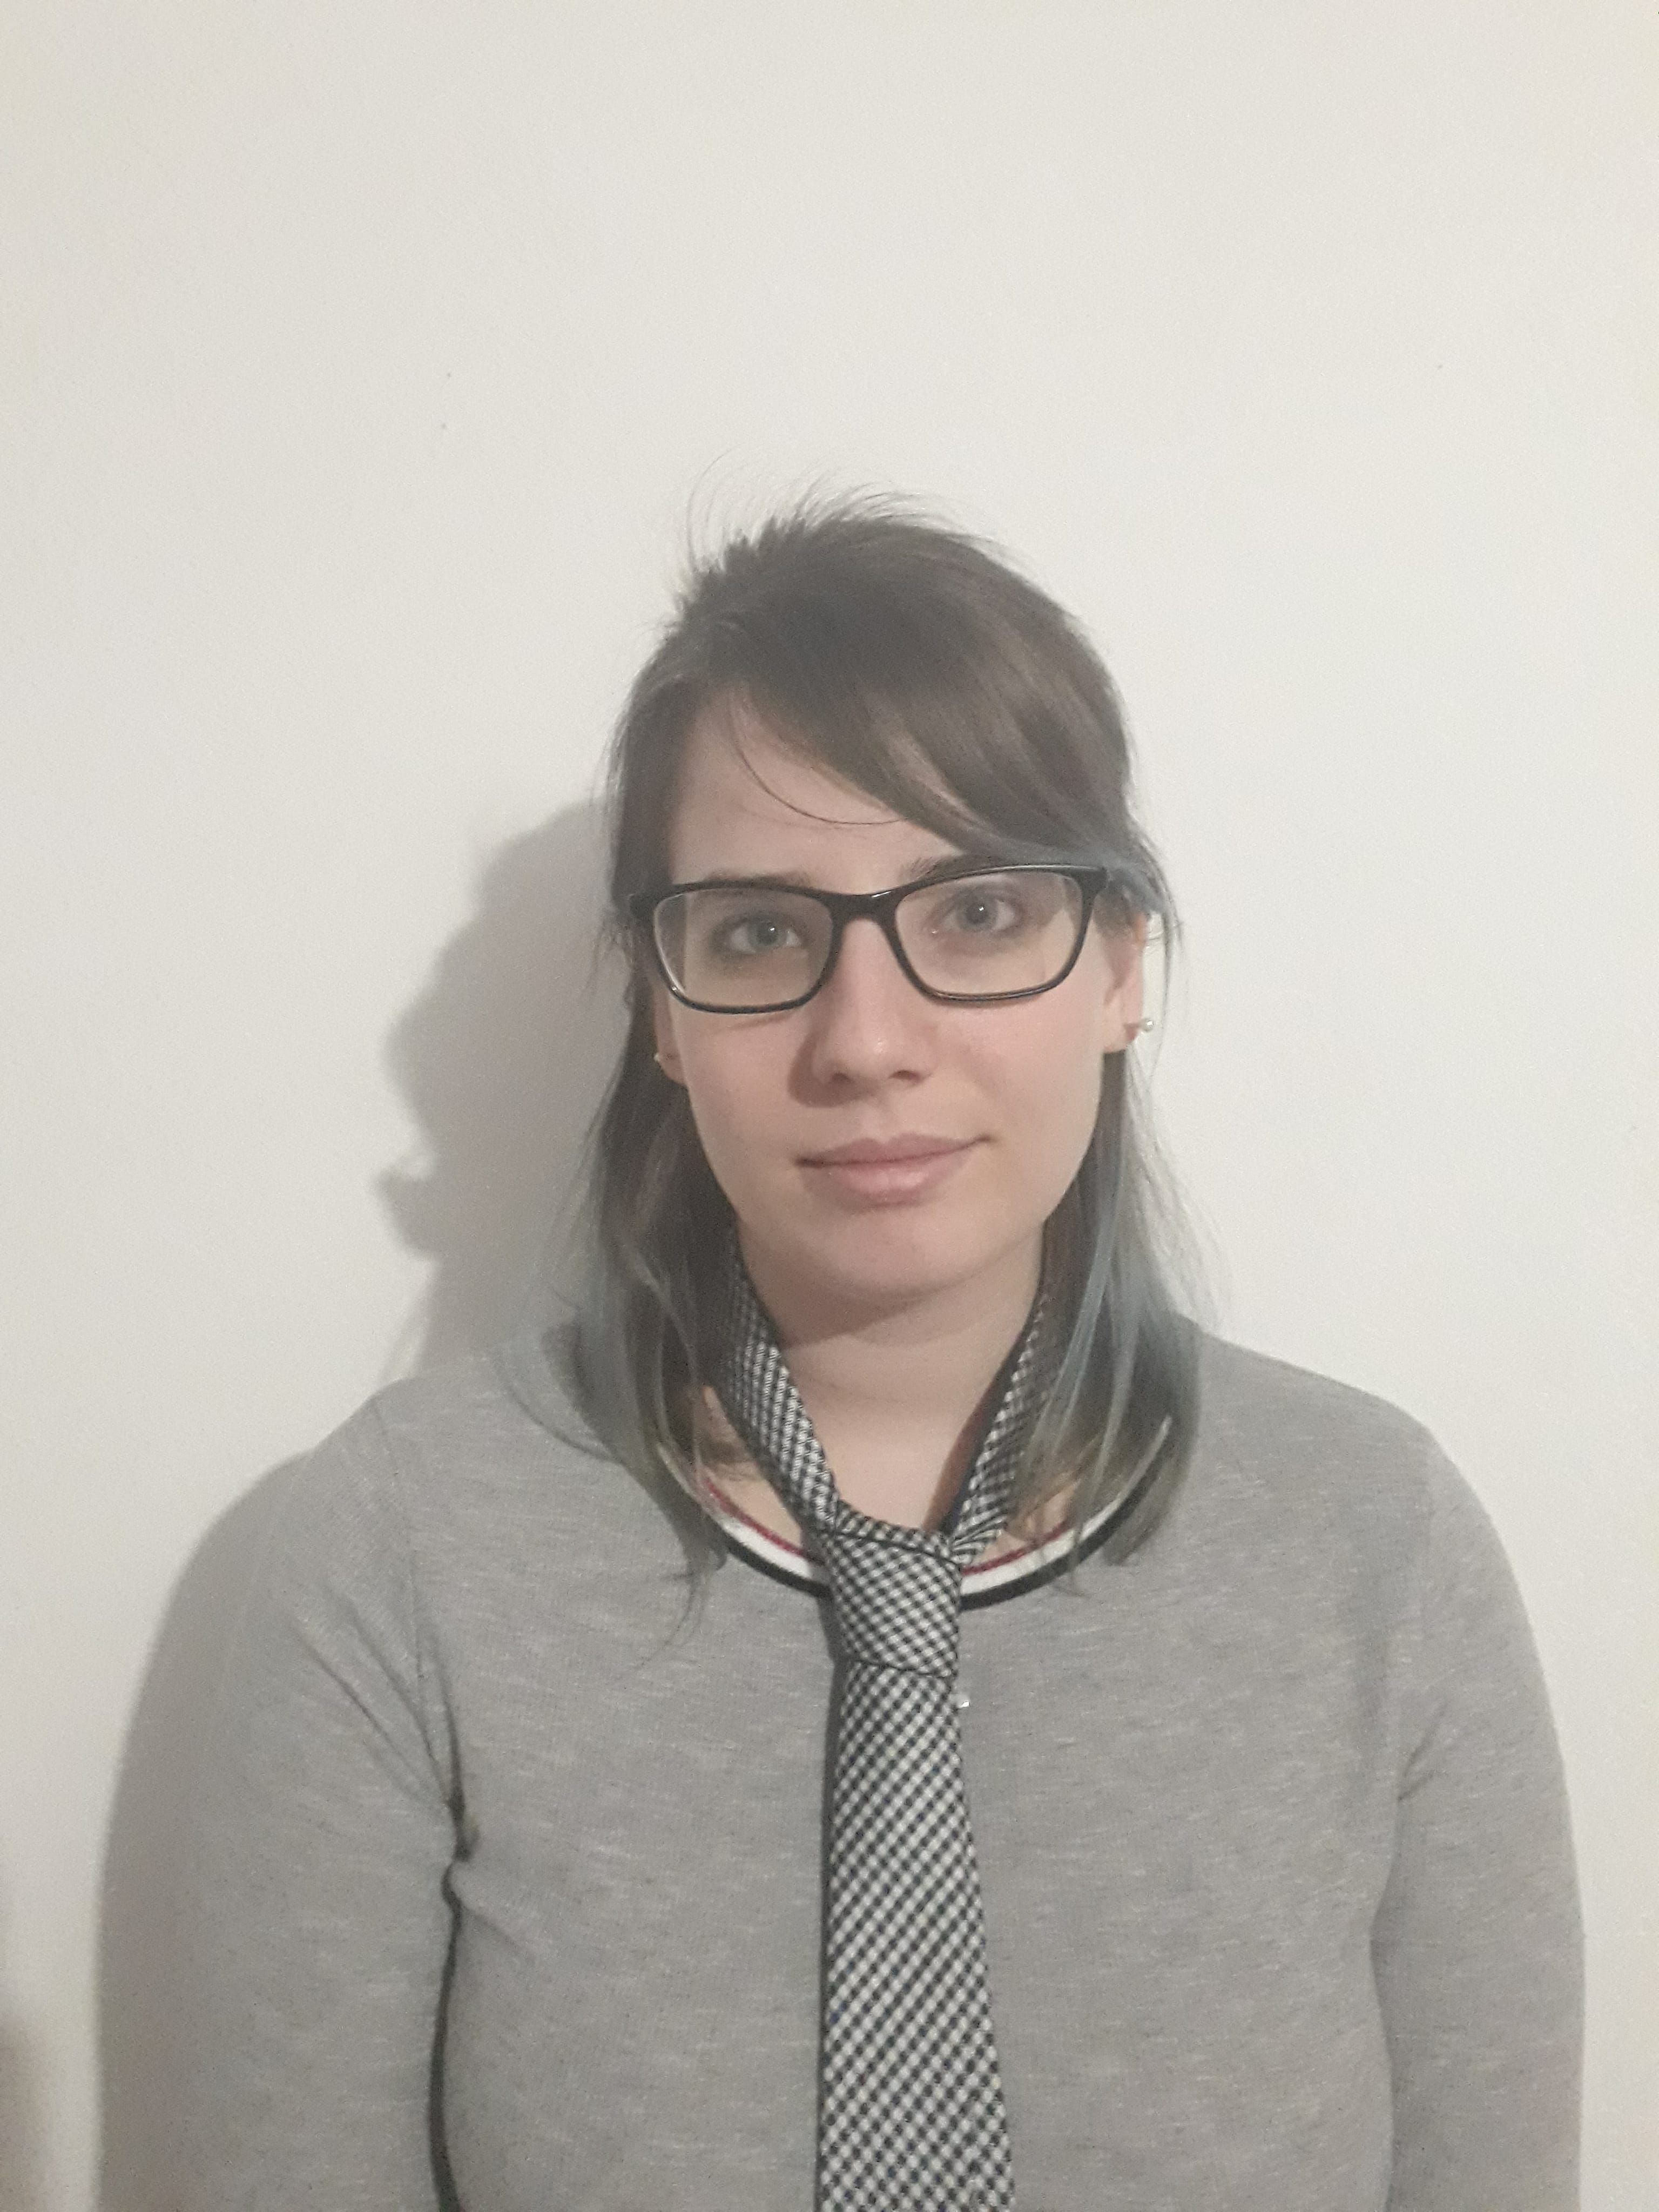
\includegraphics[scale=0.04]{images/27785203_330504664108478_1945544054_o.jpg}
        \caption{Photographie de Nathanaëlle VILLER}
    \end{figure}
En utilisant l'image de chat dans la recherche de Google Image on obtient le résultat ci dessous. (Figure 3) Nous pouvons constater qu'il retourne les sites utilisant l'image fournis et qu'il propose de chercher les images similaires.  Malheureusement, cette recherche va "traduire" en mots clefs notre image initiale pour fournir des images peu similaire. Voir Annexe 1. 

    \begin{figure}[!h]
    \centering
        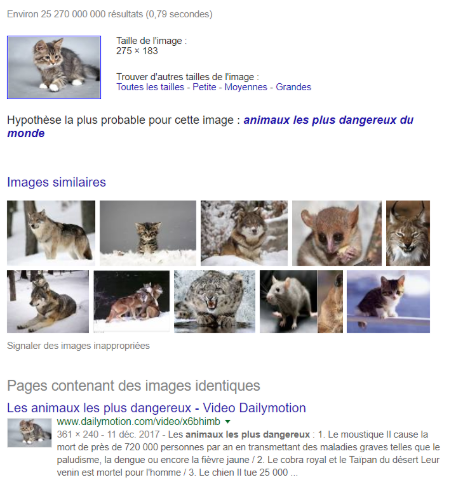
\includegraphics[scale=1]{images/ResGI.PNG}
        \caption{Résultat de la recherche via une image sur Google}
    \end{figure}

Le résultat des images similaires fournit par google avec la photographie en Figure 2 n'est pas plus concluante non plus. (Figure 4) En effet, Google va aussi "traduire" la photographie en un mot clef : girl, et ressort des images de femmes et d'hommes. Les photographies sont similaire dans leur style. On peut voir qu'il y a une personne sur un fond en général unique mais en rien ces personnes ne ressemblent à Nathanaëlle VILLER. 
    \begin{figure}[!h]
    \centering
        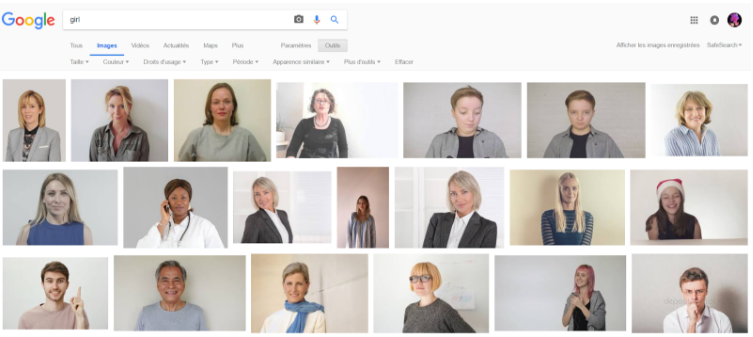
\includegraphics[scale=0.7]{images/Res3GI.PNG}
        \caption{Résultat de la recherche des images similaires par Google pour la Figure 2}
    \end{figure}
    
\subsubsection{Site de recherche de sosie}
Il existe quelques sites permettant de chercher son sosie. L'un des plus connu est twinstrangers.com. Ce site demande une photo, ainsi que quelques informations comme la date de naissance et le genre. Le site retourne ensuite la personne avec le plus de similitude. Pour accéder au suivant il faut payer. 
Voir Annexe 2 pour les 3 premiers résultats obtenus à partir de la photographie en Figure 2. 
    
Il s'agit de jeunes filles d'un âge plus ou moins proche de Nathanaëlle, leurs yeux sont également clairs et elles portent des lunettes. Mais on ne peut pas parler de sosie. 
D'après les termes d'utilisations du site nous pouvons apprendre que seul le visage (à partir de la photo) sert à faire la recherche. Cette dernière sera faite parmi la base de données du site. Rien n'est dit par rapport au genre, mais puisqu'il faut le renseigner nous pouvons nous questionner si ce dernier ne permettrai pas de faire un premier filtre. Ce site à pour but de permettre à des sosies de se trouver puis de se rencontrer. Cette plate-forme se limite à une base de données interne et à des personnes physiques, ce qui est différent de notre objectif.
Mais il semble intéressant d'étudier comment fonctionne l'algorithme de ce site. 
\\\\
Il existe d'autres sites tel que pictriev.com qui déduit si nous sommes un homme ou une femme ainsi que notre âge et nous fournis les célébrités auxquelles nous ressemblons le plus. Nous pouvons constater en annexe 3 que ce dernier n'est pas au point. Il en va de même pour celebslike.me (annexe 4). Tous les 2 sont des sites permettant de chercher son sosie parmi les personnalités connues. Encore une fois cela ne va pas avec nos objectifs. Au vu des résultats, les algorithmes d'être performant.

\subsubsection{Google Arts \& Culture}
Google Arts \& Culture est une application américaine qui permet de trouver son sosie en oeuvre d’art. Google Arts \& Culture a collaboré avec plus de 1 200 musées, galeries et institutions de 70 pays pour rendre leurs expositions accessibles à tous en ligne, sûrement aussi pour avoir une base de données interne à interroger. Malheureusement cette fonctionnalité "trouver son double dans une oeuvre d'art" de l'application n'est disponible qu'aux Etats Unis et un test n'a donc pas pu être possible. Mais nous pouvons trouver des articles qui en parle. Le fonctionnement est simple, il suffit de charger une photographie ou un autoportrait et l'algorithme va analyser les traits du visage à plus de 70 000 portraits provenant de collection du monde entier. Twitter a été rempli de test des internautes américains dont voici un exemple bluffant (Figure 5).
\begin{figure}[!h]
    \centering
        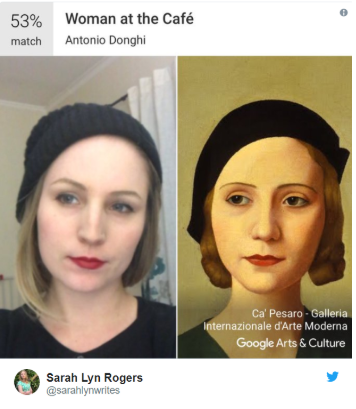
\includegraphics[scale=1]{images/GAC.PNG}
        \caption{Exemple trouvé sur Twitter}
    \end{figure}

La technologie de reconnaissance faciale FaceNet développée par Google, utilisé dans cette application est désormais disponible dans une version open-source officieuse, OpenFace. Cette dernière est très intéressantes pour notre sujet de recherche. Les résultats obtenu par l'application sont concluant et l'on observe des similitudes entres les deux photographies. Il s'agit de la première application connu permettant de trouver son sosie avec une oeuvre d'art. Ce qui rejoint fortement notre objectif bien que se limitant à des oeuvres d'art.  

\subsubsection{Les sites de rencontre}
Les sites de rencontrent se mettent de plus en plus dans la recherche de sosie. L'objectif est de permettre aux internautes de chercher un sosie de leur célébrité préférée ou de leur ex-partenaire ou de la personne leur plaisant mais étant déjà prise. Dans les sites de rencontre permettant ce genre de recherche nous pouvons citer Badoo et Match. 
Badoo est assez frappant car les similitudes trouvés sont forte (même si certains correspondent à de faux comptes usurpant la photo d'une autre personne). (Figure 6) 
\begin{figure}[!h]
    \centering
        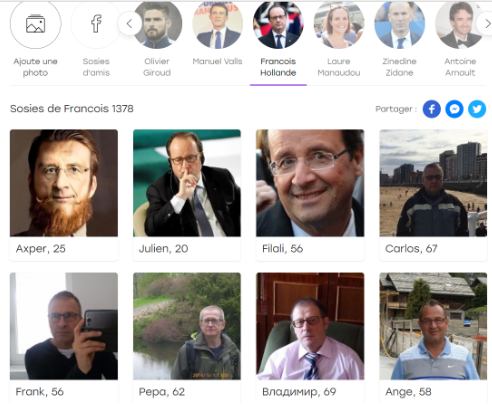
\includegraphics[scale=1]{images/badoo.PNG}
        \caption{Exemple avec Badoo}
    \end{figure}
    
\subsubsection{Conclusions sur ces solutions}

Actuellement, les solutions permettent surtout de trouver un sosie de nous mêmes avec une personne physique. Mais aucune d'entre elles n'est une solution probante. Il existe des solutions (application ou site web) mais en général elles se servent dans leur base de données locale et pas "sur internet" en règle générale. 

Ce qui manque à ces applications : 
\begin{itemize}
    \item Une recherche à travers internet 
    \item Une sortie de sosie qui ne soit pas uniquement une personne physique réelle 
    \item Une reconnaissance morphologique en plus de celle faciale
\end{itemize}

Pour ce qui est du second point, Google a développé un algorithme permettant de chercher un sosie avec une oeuvre d’art de type peinture ou dessin exposé dans un musée. Il faudrait donc trouver une solution pour proposer un outil à plus large spectre, qui reprendrait l’existant mais pour le mener plus loin. 
Ouvrir le retour de sosie à toute oeuvre : peinture, dessins, coloriage, photographie … Pour trouver une personne physique ou un personnage fictif en terme de sosie. Et, effectuer la recherche en dehors d'une base de données locale mais s'appuyer sur toutes les ressources dont disposes internet. 

\section{Solution proposée}
\section{Domaine d'application}
\newpage
\addcontentsline{toc}{section}{Conclusion}
\section*{Conclusion}


\newpage



\section{Annexes}
Annexe 1 : 
\begin{figure}[!h]
    \centering
    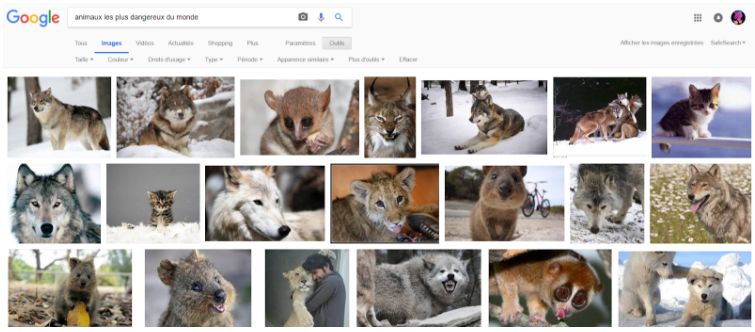
\includegraphics[scale=0.8]{images/Res2GI.PNG}
    \caption{Résultat de la recherche des images similaires par Google pour la Figure 1}
\end{figure}

Annexe 2 : 
\begin{figure}[!h]
    \centering
        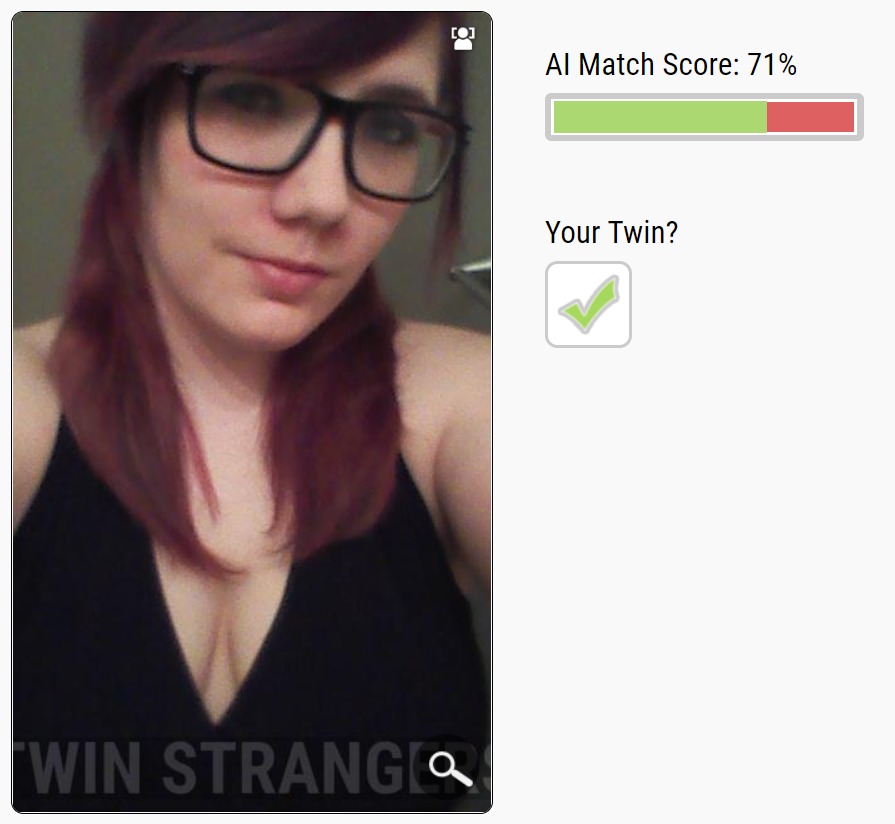
\includegraphics[scale=0.45]{images/ResS1.PNG}
        \caption{Premier sosie}
    \end{figure}
    \begin{figure}[!h]
    \centering
        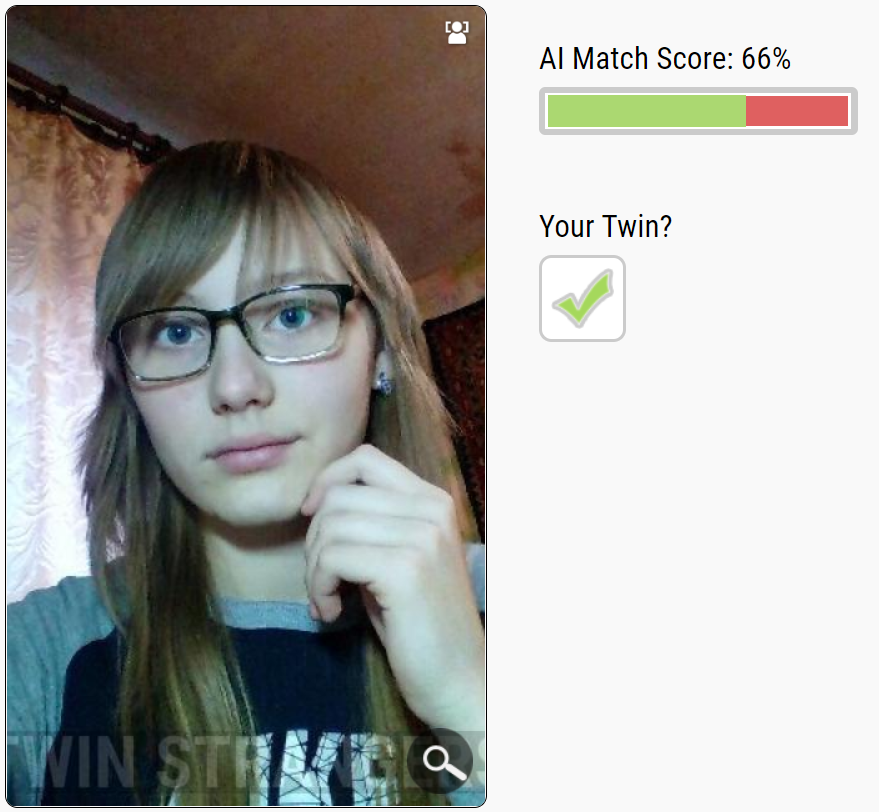
\includegraphics[scale=0.3]{images/ResS12.PNG}
        \caption{Deuxième sosie}
    \end{figure}
\begin{figure}[!h]
    \centering
        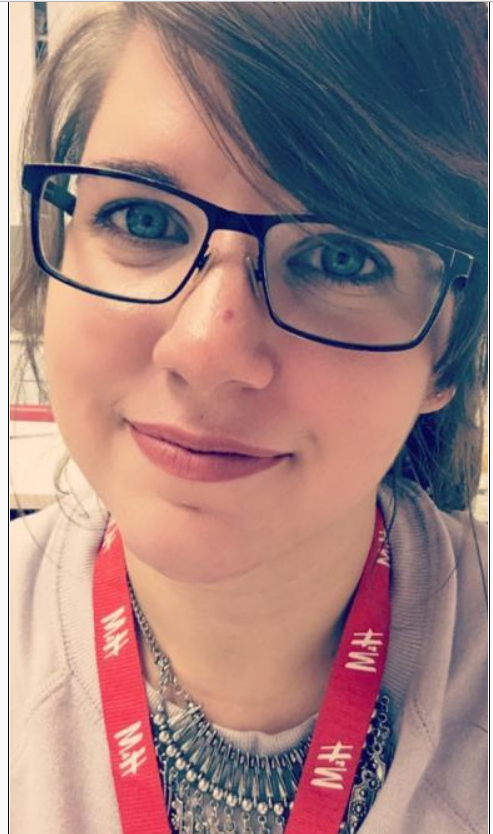
\includegraphics[scale=0.3]{images/ResS13.PNG}
        \caption{Troisième sosie}
    \end{figure}
    
  \newpage
Annexe 3 : 
\begin{figure}[!h]
    \centering
        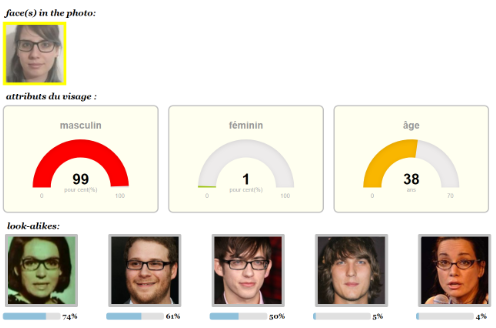
\includegraphics[scale=1]{images/ResS2.PNG}
        \caption{Résultat du second site}
    \end{figure} 
\newpage
Annexe 4 :
\begin{figure}[!h]
    \centering
        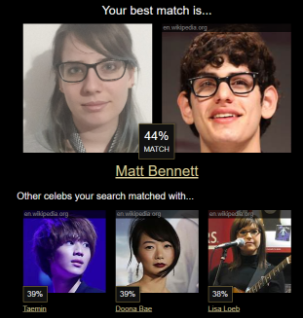
\includegraphics[scale=1]{images/ResS3.PNG}
        \caption{Résultat du troisième site}
    \end{figure}

%\subsection{}
%\subsubsection{}

%\begin{itemize}
%\item	
%\item	
%\item
%\item	
%\item	
%\end{itemize}


%\begin{center}
%		    \includegraphics[scale=0.6]{images/cas_utilisation}	
%		\end{center}
	


%\begin{verbatim}

\end{document}
